%
% dgleichverteilung.tex -- Abschnitt ueber diskrete Gleichverteilung in Kapitel 5
%
% (c) 2015 Prof Dr Andreas Mueller, Hochschule Rapperswil
%
\subsection{Gleichverteilung} \label{section-gleichverteilung-diskret}
\index{Gleichverteilung!Erwartungswert}
\index{Gleichverteilung!Varianz}
\index{Gleichverteilung!Verteilungsfunktion}
\begin{table}
\renewcommand{\arraystretch}{1.5}
\begin{center}
\begin{tabular}{|l|l|}
\hline
Name&Diskrete Gleichverteilung\\
\hline
Wahrscheinlichkeit&
\begin{minipage}{3.7in}
\vskip3pt
$\displaystyle P(k)=\frac1n$
\end{minipage}
\\
Verteilungsfunktion&
\begin{minipage}{3.7in}
$\displaystyle
\begin{cases}
0&\qquad x \le 1\\
{\displaystyle \frac{\left\lfloor x\right\rfloor}n}&\qquad 1\le x\le n
\\
1&\qquad x \ge n
\end{cases}
$
\end{minipage}
\\[30pt]
Erwartungswert&$\displaystyle \frac{n+1}2$\\[8pt]
Varianz&$\displaystyle \frac{n^2-1}{12}$\\[8pt]
Median&$\displaystyle \frac{n+1}2$\\[8pt]
\hline
Anwendungen&\begin{minipage}{3.7in}%
\vskip3pt
\strut
$\bullet$ Laplace-Ereignisse aller Art\\
$\bullet$ Würfel\\
$\bullet$ Roulette
\strut
\end{minipage}\\[17pt]
\hline
\end{tabular}
\end{center}
\caption{Datenblatt der diskreten Gleichverteilung\label{datenblatt:diskretegleichverteilung}}
\end{table}

\begin{figure}
\centering
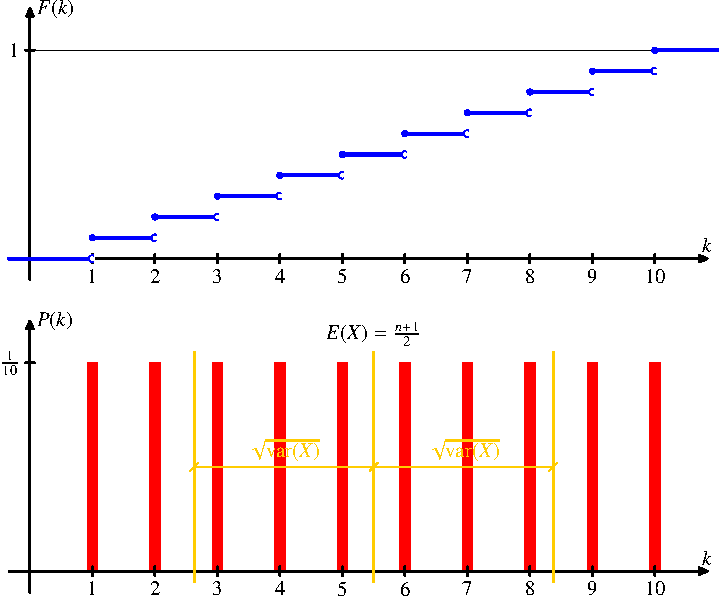
\includegraphics{images/gl-2.pdf}
\caption{Wahrscheinlichkeit und Verteilungsfunktion der diskreten Gleichverteilung
für $n=10$
\label{graph-diskrete-gleichverteilung}}
\end{figure}

Bereits in Abschnitt \ref{section-laplace-ereignisse}
wurden Ereignisse
untersucht, bei denen alle Elementarereignisse mit gleicher Wahrscheinlichkeit
eingetreten sind.
Im Kontext einer Zufallsvariable bedeutet
Gleichverteilung, dass jeder mögliche Wert mit gleicher Wahrscheinlichkeit
vorkommt.
Im einfachsten Fall sind die Werte natürliche Zahlen
$\{1,\dots,n\}$, die Wahrscheinlichkeit für den Wert ist 
$p(k)=\frac1n$.
Die Verteilungsfunktion dieser Verteilung ist
\[
F(x)=
\begin{cases}
0&\qquad x \le 1\\
{\displaystyle \frac{\left\lfloor x\right\rfloor}n}&\qquad 1\le x\le n\\
1&\qquad x \ge n
\end{cases}
\]
Entsprechend einfach sind Erwartungswert und Varianz zu berechnen:
{\allowdisplaybreaks
\begin{align*}
E(X)&=\sum_{k=1}^nkp(k)=\frac1n\sum_{k=1}^nk=\frac1n\cdot\frac{n(n+1)}{2}=\frac{n+1}2\\
E(X^2)&=\sum_{k=1}^nk^2p(k)=\frac1n\sum_{k=1}^nk^2=\frac1n\cdot\frac{n(1+3n+2n^2)}{6}=\frac{2n^2+3n+1}{6}\\
\operatorname{var}(X)&=E(X^2)-E(X)^2=\frac{2n^2+3n+1}{6}-\frac{(n+1)^2}4\\
&=\frac{4n^2+6n+2-3n^2-6n-3}{12}=\frac{n^2-1}{12}
\end{align*}
}
Die Wahrscheinlichkeit und die Verteilungsfunktion ist in
Abbildung~\ref{graph-diskrete-gleichverteilung} dargestellt.
